In this Section, starting from the measurement process, we establish a
statistical model for curb detection and derive appropriate inference
algorithms.

\subsection{Measurement Representation}

A nodding laser range-finder produces scan measurements $\mathbf{s}_i=[r_i,
\theta_i,\psi_i]^\text{T}$ that are transformed into their corresponding
Cartesian 3D coordinates $\mathbf{p}_i=[x_i,y_i,z_i]^\text{T}$, where $r_i$ is
a range measurement, $\theta_i$ a pitch angle, and $\psi_i$ a bearing angle. The
sensing device has an error model which is typically a function of
$\mathbf{s}_i$. From a complete laser sweep, we obtain a point cloud
representation $\mathcal{P}=\{\mathbf{p}_1,\mathbf{p}_2,\dots,\mathbf{p}_N\}$.

Unfortunately, point clouds are inconvenient models in the context of robot
navigation, where single points are frequently subject to expensive random
access operations, e.g., in the case of collision checks. Therefore, it will be
beneficial to project $\mathcal{P}$ onto a 2D grid
$\{\mathcal{C}_1,\mathcal{C}_2,\dots,\mathcal{C}_M\}$, with cells
$\mathcal{C}_i=\{\mathbf{c}_i,\mathbf{B}_i,h_i\}$, where
$\mathbf{c}_i=[c_{i_x},c_{i_y}]^\text{T}$ is the cell center,
$\mathbf{B}_i=[\mathbf{ul}_i, \mathbf{lr}_i]^\text{T}$ its bounding box with
upper left point $\mathbf{ul}_i$ and lower right point $\mathbf{lr}_i$, $h_i$
its height.

To account for the noise induced by the aforementioned measurement and
discretization process, we model the height $h_i$ as a normal distribution
$p(h_i\mid\mu_{h_i},\sigma^2_{h_i})=\mathcal{N}(h_i\mid\mu_{h_i},
\sigma^2_{h_i})$, with mean $\mu_{h_i}$ and variance $\sigma^2_{h_i}$ to be
estimated. To this end, we collect the set of points $\mathcal{I}_i=\{z_j\mid
\mathbf{p}_j\in\mathcal{P}, [x_j,y_j]^\text{T}\subset\mathbf{B}_i\}$ and adopt a
purely Bayesian approach~\cite{gelman03bayesian}. This involves setting a joint
prior $p(\mu_{h_i},\sigma^2_{h_i})$ over the parameters, computing the
posterior $p(\mu_{h_i},\sigma^2_{h_i}\mid\mathcal{I}_i)$, and ultimately
formulating a posterior predictive density $p(\mu_{h_i}\mid\mathcal{I}_i)$ that
will be subsequently termed our \emph{cell model}. We choose a conjugate
normal inverse-gamma prior that incorporates the sensor and discretization noise
in its hyperparameters. The resulting posterior predictive density is thus a
Student's t-distribution. We denote the mean and variance of this density
$\hat{\mu}_{h_i}$ and $\hat{\sigma}^2_{h_i}$ respectively. Apart from its
elegance, this Bayesian method can plainly reflect our noise model and remains
robust to outliers, especially in case of few measurements.

In the literature, the 2D grid employed in this paper is commonly designated a
\emph{Digital Elevation Map} (DEM). We will therefore adopt the notion and
henceforth use it to refer to this kind of grid. The choice of a DEM
representation is mainly guided by the application scope of the algorithm. It
may for example be interpreted as a traversability map for the planning process.
It is furthermore convenient for defining Regions of Interest (ROI) in
$\mathcal{P}$ and for facilitating further computations. Finally, it provides
constant-time lookup to the cells, either addressed by their geometrical
coordinates or row-column indices. We shall discuss later on the issue of
cell discretization. Fig.~\ref{fig:dem} displays an example of a DEM from a 3D
point cloud.

\begin{figure}[t]
\centering
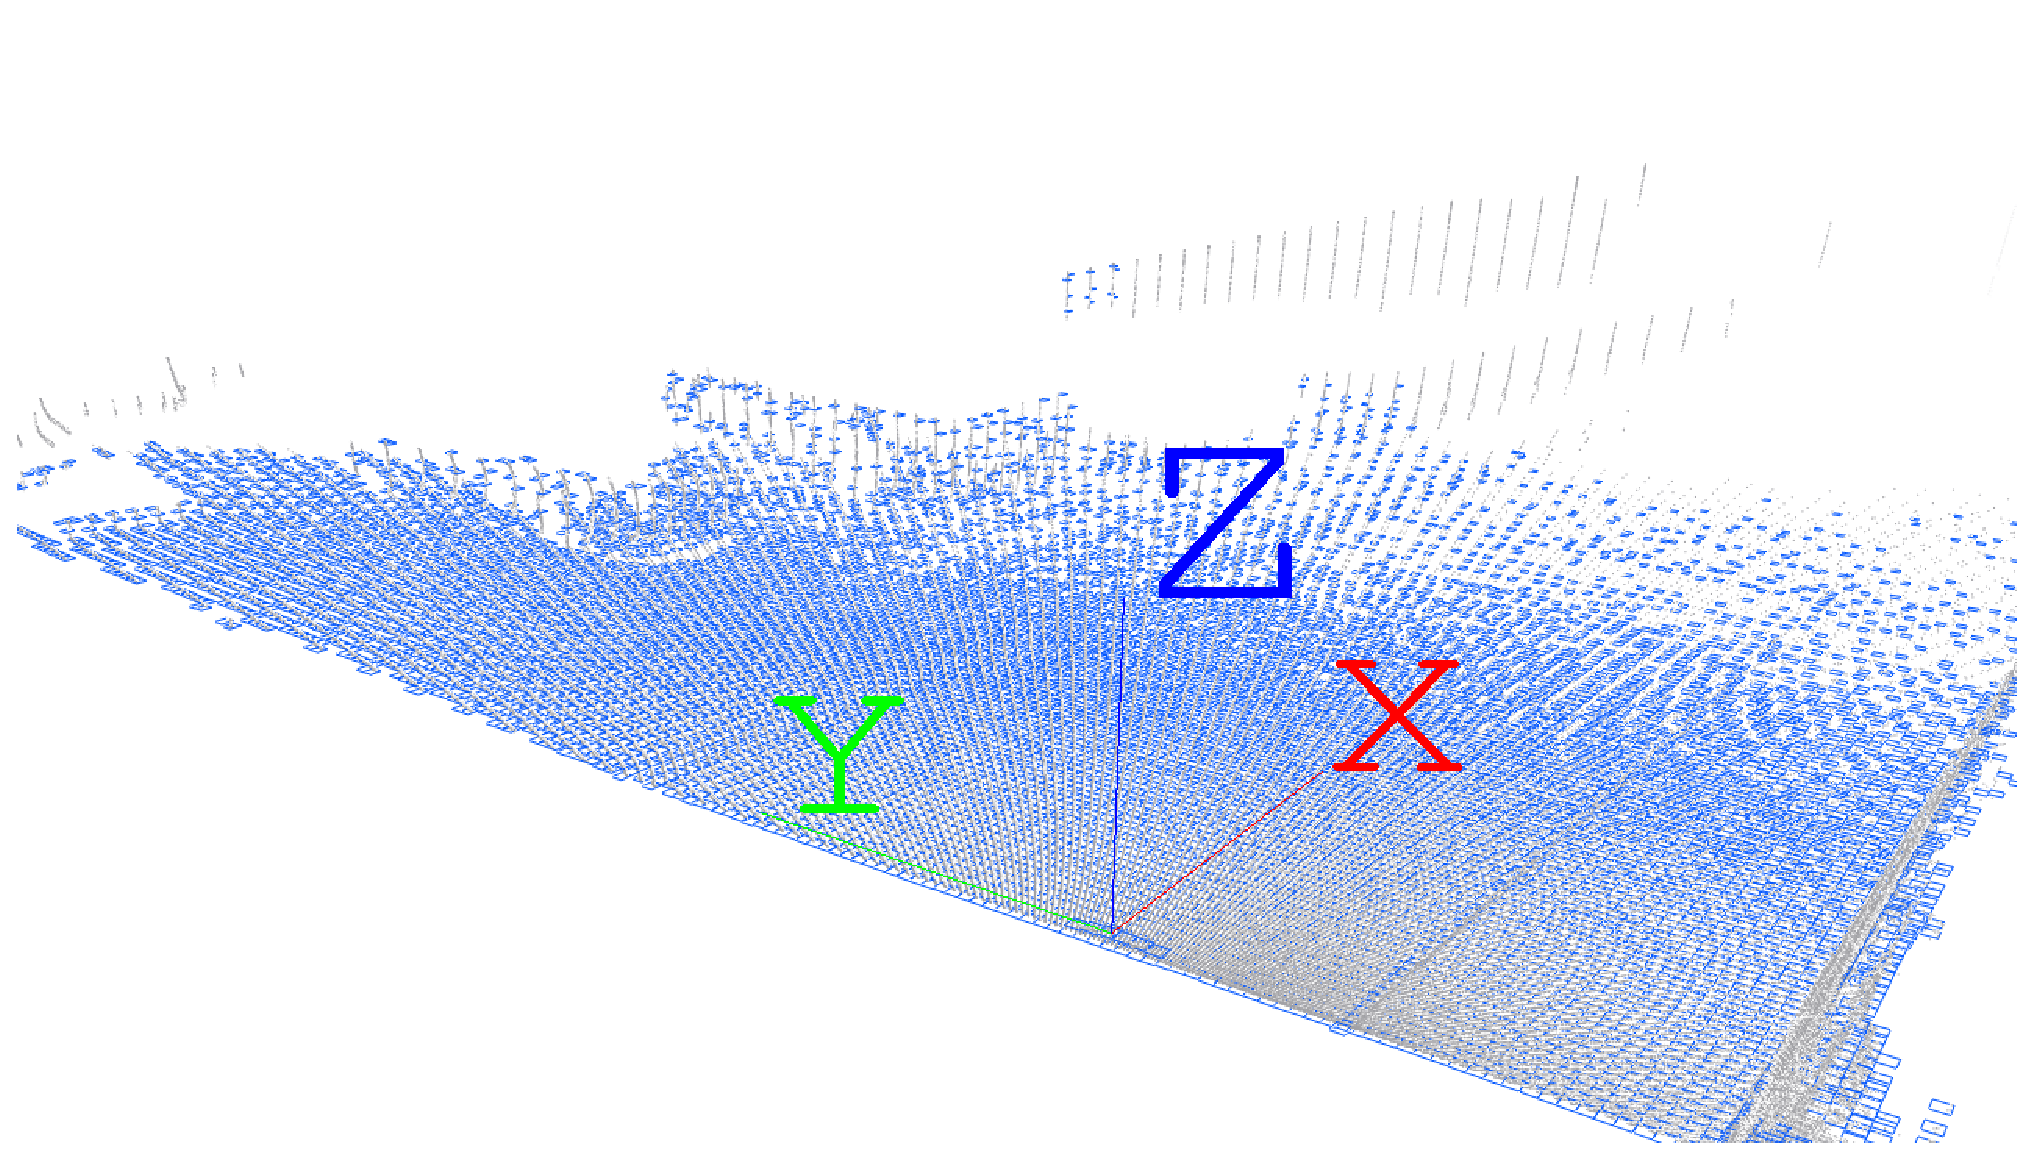
\includegraphics[width=\columnwidth]{fig/dem.eps}
\caption{A 3D point cloud (gray) is represented as a Digital Elevation Map (DEM)
(blue), i.e., a projection of the points into 2D grid cells using Bayesian
inference. The means $\hat{\mu}_{h_i}$ of the posterior predictive distributions
are displayed here for the cell height values.}
\label{fig:dem}
\end{figure}

\subsection{Environment Model and Inference Task}

We assume a piecewise planar environment, i.e., the observed scene is composed
of a set of plane segments. Boundaries between plane segments define local
height discontinuities that we shall henceforth term \emph{curbs}.
Fig.~\ref{fig:model} depicts a typical environment model.

\begin{figure}[t]
\centering
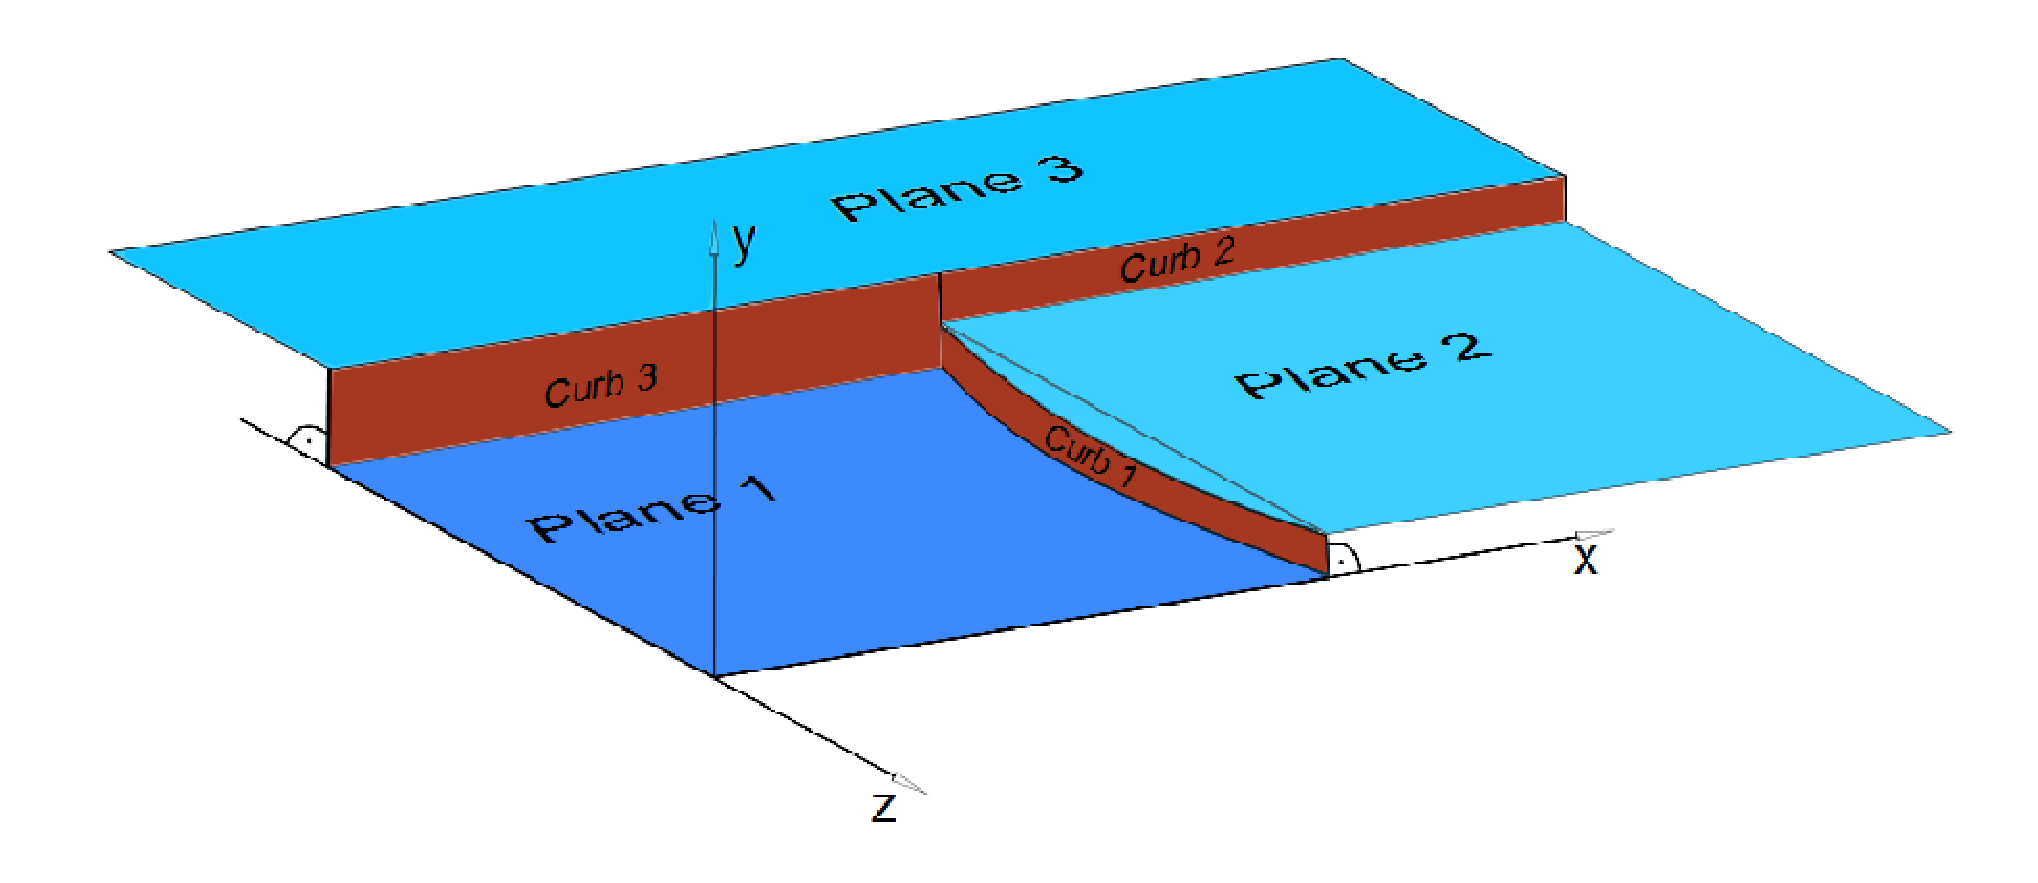
\includegraphics[width=\columnwidth]{fig/model.eps}
\caption{The proposed environment model is composed of a set of plane segments.
Curbs are defined as the boundaries between plane segments.}
\label{fig:model}
\end{figure}

On the one hand, the major inference task therefore boils down to discovering
those plane segments, and on the other hand, to determining the assignment of
the DEM cells to these latter. To this end, we model the environment with a
conditional mixture model, namely a \emph{mixture of linear regression} model.
According to the discussions in~\cite{bishop06pattern}, we may thus state the
following generative process for the mean height values:

\begin{equation}
\label{eqn:mixture}
p(\hat{\mu}_{h_i}\mid\mathbf{c}_i, \Theta)=\sum_{k=1}^K\pi_k\mathcal{N}
(\hat{\mu}_{h_i}\mid\mathbf{w}_k^\text{T}\boldsymbol{\phi}(\mathbf{c}_i),
\sigma^2_k),
\end{equation}

where $\Theta=\{\boldsymbol{\pi},\mathbf{W},\boldsymbol{\sigma}^2\}$ is the set
of adaptive parameters to be estimated, $\boldsymbol{\pi}=\{\pi_k\}$ are the
mixture weights, $\mathbf{W}=\{\mathbf{w}_k\}$ the regression coefficients,
$\boldsymbol{\sigma}^2=\{\sigma^2_k\}$ the regression variances, and
$\boldsymbol{\phi}(\mathbf{c}_i)=[1\;\mathbf{c}_i]^\text{T}$ the explanatory
variables or \emph{covariates}. The cell variance $\hat{\sigma}^2_{h_i}$ can
be introduced in the parameter estimation as we shall demonstrate below.

For solving the classification task, we introduce an additional categorical
latent variable $\mathbf{l}_i$, which has a 1-of-K representation such that
its prior distribution is defined as $p(l_{i_k}=1)=\pi_k$. Intuitively, the
posterior distribution $p(l_{i_k}=1\mid\hat{\mu}_{h_i})$ or
\emph{responsibility} $\gamma_{ik}$ represents the probability for the cell
$\mathcal{C}_i$ to belong to plane $k$.

\subsection{Parameter Estimation}

Given an instance of a DEM, the parameter set $\Theta$ of the mixture model has
to be estimated. We adopt here a Maximum-Likelihood (ML) approach, i.e., we
search for the parameters $\hat{\Theta}$ that maximize the likelihood function
or "best" explain the data.

We define the vector of all mean height values as $\hat{\boldsymbol\mu}_h=
[\hat{\mu}_{h_1}\dots\hat{\mu}_{h_M}]^\text{T}$, the matrix of covariates as
$\boldsymbol{\Phi}=[\boldsymbol{\phi}(\mathbf{c}_1)\dots\boldsymbol{\phi}
(\mathbf{c}_{M})]^\text{T}$, and the matrix of latent variables as
$\mathbf{L}=[\mathbf{l}_1\dots\mathbf{l}_M]^\text{T}$. Due to singularities,
there is no analytical solution to the direct maximization of the likelihood
function $p(\hat{\boldsymbol\mu}_h\mid\Theta,\boldsymbol{\Phi})$. An
Expectation-Maximization (EM) algorithm~\cite{dempster77maximum} is the
prevalent choice in the literature for solving this kind of problem. If, for
each point, we were given its class assignment, i.e., we would observe a
\emph{complete} data set, the maximization of the complete-data likelihood
$p(\hat{\boldsymbol\mu}_h,\mathbf{L}\mid\Theta,\boldsymbol{\Phi})$ would be
simplified. Although latent variables are not observed, we can compute their
posterior distribution $p(\mathbf{L}\mid\Theta^\text{old},\boldsymbol{\Phi})$
using an initial parameter estimate $\hat{\Theta}^{(t)}$. In the E-step of
the EM algorithm, the expectation of the complete-data likelihood under this
posterior is firstly calculated. In the M-step, a new parameter set
$\hat{\Theta}^{(t+1)}$ is obtained by maximization of this likelihood.
The algorithm iterates between these steps until convergence of the likelihood.

More specifically, in a standard EM for mixture of linear regression model, we
compute responsibilities $\gamma_{ik}$, or posterior class assignments, using
Bayes rule in the E-step with

\begin{equation}
\label{eqn:responsibility}
p(l_{i_k}=1\mid\hat{\mu}_{h_i},\mathbf{c}_i,\hat{\Theta}^{(t)})=\gamma_{ik}
\propto\pi_k\mathcal{N}(\hat{\mu}_{h_i}\mid\mathbf{w}_k^\text{T}
\boldsymbol{\phi}(\mathbf{c}_i),\sigma^2_k).
\end{equation}

Here, the attentive reader shall have noticed that we have used conditional
independence of the $\mathbf{l}_i$ given the data, that is:

\begin{equation}
\label{eqn:factorization}
p(\mathbf{L}\mid\hat{\boldsymbol\mu}_h,\boldsymbol{\Phi},\hat{\Theta}^{(t)})
=\prod_{i=1}^M p(\mathbf{l}_i\mid\hat{\mu}_{h_i},\mathbf{c}_i,
\hat{\Theta}^{(t)}).
\end{equation}

In the M-step of the algorithm, the maximization yields the following parameter
estimates $\hat{\Theta}^{(t+1)}$:

\begin{equation}
\label{eqn:coeff}
\mathbf{w}_k = (\boldsymbol{\Phi}^\text{T}\mathbf{R}_k\boldsymbol{\Phi})^{-1}
\boldsymbol{\Phi}^\text{T}\mathbf{R}_k\hat{\boldsymbol\mu}_h,
\end{equation}

\begin{equation}
\label{eqn:numpoints}
N_k = \sum_{i=1}^M\gamma_{ik},
\end{equation}

\begin{equation}
\label{eqn:var}
\sigma^2_k = \frac{1}{N_k}(\hat{\boldsymbol\mu}_h-\boldsymbol{\Phi}
\mathbf{w}_k)^\text{T}(\hat{\boldsymbol\mu}_h-\boldsymbol{\Phi}\mathbf{w}_k),
\end{equation}

\begin{equation}
\label{eqn:weights}
\pi_k = \frac{N_k}{M},
\end{equation}

where $\mathbf{R}_k=\text{diag}(\gamma_{ik})$ contains the responsibilities for
component $k$ in a diagonal matrix.

\subsection{Belief Propagation for Posterior Class Assignments}

As we have pointed out in \eqref{eqn:factorization}, the computation of the
joint posterior class assignment
$p(\mathbf{L}\mid\hat{\boldsymbol\mu}_h,\boldsymbol{\Phi},\hat{\Theta}^{(t)})$
can be handled independently for each $\mathbf{l}_i$ in the standard EM
algorithm. The sought marginals $\gamma_{ik}$ are therefore straightforwardly
calculated. However, the nature of our problem suggests that we should introduce
dependencies between neighboring DEM cells. Indeed, geometrically close points
are more likely to lie in the same plane. We hence define an undirected graph
$\mathcal{G}=\{\mathcal{V},\mathcal{E}\}$, with vertices $v_i\in\mathcal{V}$ and
edges $(v_i,v_j)\in\mathcal{E}$ connecting neighboring vertices. Each DEM cell
$\mathcal{C}_i$ is assigned to a vertex $v_i$ having a 4-connected neighborhood.

Borrowing in the literature of graphical models, we can express the joint
posterior class assignment factorization with a Conditional Random Field
(CRF)~\cite{lafferty01conditional} on the graph $\mathcal{G}$ as:

\begin{eqnarray}
\label{eqn:crf_joint}
p(\mathbf{L}\mid\hat{\boldsymbol\mu}_h,\boldsymbol{\Phi},\hat{\Theta}^{(t)})
\propto
\phantom{aaaaaaaaaaaaaaaaaaaaaaaaaaaa}\\ \nonumber
\prod_{v_i\in\mathcal{V}}
\varphi_i(\hat{\mu}_{h_i},\mathbf{l}_i,\hat{\Theta}^{(t)},\boldsymbol{\Phi})
\prod_{(v_i,v_j)\in\mathcal{E}}\psi_{ij}(\hat{\mu}_{h_i},\hat{\mu}_{h_j},
\mathbf{l}_i,\mathbf{l}_j),
\end{eqnarray}

where $\varphi_i(\cdot)$ and $\psi_{ij}(\cdot)$ are the \emph{node potentials}
and \emph{edge potentials} respectively. The potential functions are positively
defined functions and the normalization is ensured by the
\emph{partition function} $\mathbf{Z}(\boldsymbol{\Phi})$. Intuitively, a node 
potential reflects the likelihood of $\hat{\mu}_{h_i}$ being labeled
$\mathbf{l}_i$, and an edge potential the joint likelihood of $\hat{\mu}_{h_i}$
and $\hat{\mu}_{h_j}$ being labeled $\mathbf{l}_i$ and $\mathbf{l}_j$.

Given the formulation in \eqref{eqn:crf_joint}, two inference tasks are of
interest. On the on hand, one can derive the marginals
$p(\mathbf{l}_i\mid\hat{\mu}_{h_i},\mathbf{c}_i,\hat{\Theta}^{(t)})$, and on the
other hand, one can find the Maximum A Posteriori (MAP) joint state
$\mathbf{L}^\text{MAP}$ of the CRF. The former question is addressed with the
sum-product algorithm, while the latter with the max-product, which give exact
results for tree. These are two instances of Belief Propagation (BP). Even
though our graph $\mathcal{G}$ contains loops, BP can yield approximate
results~\cite{mooij07sufficient} and is in this case called \emph{loopy} BP.
Fig.~\ref{fig:fg} shows an excerpt of the factor
graph~\cite{kschischang01factor} on which the inference operates.

\begin{figure}[t]
\centering
\begin{tikzpicture}
\node [matrix,matrix anchor=mid, column sep=20pt, row sep=10pt] {
&\node (l0) [latent] {$\mathbf{l}_0$};
&\node (l01) [factor] {$\psi_{01}$};
&\node (l1) [latent] {$\mathbf{l}_1$};
&\node (l12) [factor] {$\psi_{12}$};
&\node (l2) [latent] {$\mathbf{l}_2$};
&\node (la) [factor] {$\psi_{\dots}$};&\\
};
\node (l0fac) [factor, above=12pt of l0] {$\varphi_0$};
\node (l1fac) [factor, above=12pt of l1] {$\varphi_1$};
\node (l2fac) [factor, above=12pt of l2] {$\varphi_2$};
\draw [-] (l0) -- (l0fac);
\draw [-] (l1) -- (l1fac);
\draw [-] (l2) -- (l2fac);
\draw [-] (l0) -- (l01);
\draw [-] (l01) -- (l1);
\draw [-] (l1) -- (l12);
\draw [-] (l12) -- (l2);
\draw [-] (l2) -- (la);
\end{tikzpicture}
\caption{Excerpt of the factor graph used for Belief Propagation (BP). Latent
variables ($\mathbf{l}_i$) are displayed with circles and factor nodes
($\psi_{ij}$,$\varphi_i$) with squares. The factor graph expresses our specific
joint factorization.}
\label{fig:fg}
\end{figure}

We express the node potentials as follows:

\begin{equation}
\label{eqn:node_potential}
\varphi_i(\hat{\mu}_{h_i},\mathbf{l}_i,\hat{\Theta}^{(t)},\boldsymbol{\Phi})=
\pi_k\mathcal{N}(\hat{\mu}_{h_i}\mid\mathbf{w}_k^\text{T}
\boldsymbol{\phi}(\mathbf{c}_i),\sigma^2_k).
\end{equation}

We note here that the CRF does not require a normalized potential. Apart from
the normalizer, this expression is similar to \eqref{eqn:responsibility}. As
expected, BP will hence converge to the same marginals $\gamma_{ik}$ if edge
potentials are omitted.

In analogy to the approach presented in~\cite{siegemund10curb}, we express the
inter-node dependencies by means of two symmetric sigmoid functions. Therefore,
we define the edge potentials as

\begin{eqnarray}
\label{eqn:edge_potential}
\psi_{ij}(\hat{\mu}_{h_i},\hat{\mu}_{h_j},\mathbf{l}_i,\mathbf{l}_j)=
\phantom{aaaaaaaaaaaaaaaaaaaaaaa}\\\nonumber
\left\{
\begin{array}{l l}
1-(1+\exp(\sigma^2_{ij}-d_{ij}))^{-1} & \quad
\text{if $\mathbf{l}_i=\mathbf{l}_j$}\\
(1+\exp(\sigma^2_{ij}-d_{ij}))^{-1} & \quad
\text{otherwise},
\end{array} \right.
\end{eqnarray}

where $d_{ij}=|\hat{\mu}_{h_i}-\hat{\mu}_{h_j}|$ is the absolute mean height
difference between the neighboring cells $\mathcal{C}_i$ and $\mathcal{C}_j$.
Additionally, $\sigma^2_{ij}=\hat{\sigma}^2_{h_i}+\hat{\sigma}^2_{h_j}$
represents the sum of the involved measurement variances. Consequently, we
account for the errors in both cell models $\hat{\sigma}^2_{h_i}$ and
$\hat{\sigma}^2_{h_j}$.
